% !TeX spellcheck = de_DE
\documentclass[.../Dokumentation.tex]{subfiles}
\begin{document}
\subsection{Ergebnis}\label{sec-ita1-result}
Obwohl die in \ref{sec-ita1-cars} gezeigte Skizze die Dimensionen der zu 
installierenden Komponenten genau berücksichtigte, war der im Inneren des 
Fahrzeugs vorgesehene Platz nicht ausreichend bemessen.
Zu sehen ist diese Abweichung in Abbildung \ref{fig-car-too-small}.
Der Grund hierfür ist, dass die Spezifikationen des gewählten Akkus nicht 
berücksichtigten, dass der Akku selbst zusätzlich in einer schützenden Hülle 
verpackt ist. 
Um diese Hülle nicht entfernen zu müssen, wurden die 
Maße der Aussparung im Inneren des Fahrzeugs angepasst. Dadurch ergab 
sich weiter der Bedarf, diesen Zuwachs auch auf die Außenmaße anzuwenden. 
Außerdem wurde deutlich, dass das beispielsweise für die Radkästen benötigte
Stütz\-material auch in den Hohlräumen der Befestigungsvorrichtung 
eingesetzt wurde. \textit{Cura} verfügt nicht über die Option, Stützmaterial nur 
punktuell einzusetzen. Es wird entweder an jeder ermittelten Stelle verwendet 
oder an keiner. 
\begin{figure}[H]
    \begin{center}
    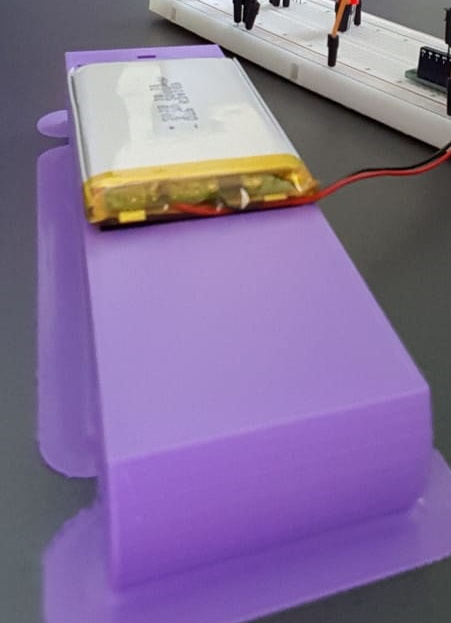
\includegraphics[
        width=0.5\linewidth,
    ]{imgs/car_too_small.jpg}
    \caption{Abweichende Maße des Akkus durch Hülle}
    \label{fig-car-too-small}
    \end{center}
\end{figure}
\noindent
Durch die Wahl einer abstrakteren Art der Darstellung besteht die Möglichkeit, 
dass der persönliche Bezug des Nutzers zu den simulierten Emissionen verloren 
geht.
Die in \ref{sec-concept} zur Sprache gekommene Unterlage verliert so, den damit 
verbundenen Aufwand berücksichtigend, an Wert.
Obwohl also durch die Umsetzung mit Hall-Sensoren 
eine recht präzise Messung der zurückgelegten Distanz möglich gewesen wäre, 
fiel an dieser Stelle die Entscheidung, auf jedwede Art von Untergrund 
für die Fahrzeuge zu verzichten. 
Beim Testen der Fahrzeugschaltung wurde festgestellt, dass die Kombination aus Pegelwandler und dem Pull-Up Widerstand nicht funktioniert und kein Auslesen von Sensorwerten möglich ist.
\end{document}